\addcontentsline{toc}{section}{Introduction}
\section*{Introduction}

Dans ce chapitre, nous discuterons du cheminement de la solution proposée pour répondre aux besoins identifiés. Nous aborderons les différentes composantes de la solution, à savoir la partie data, le backend et le frontend.

\section{Côté Data}
Dans le cadre de notre solution, nous proposons de remplacer l'exporter worker existant et les bases de données MariaDB par l'utilisation de Delta Lake sur le Cloud Object Store. Delta Lake est un système de gestion de données open-source qui offre des fonctionnalités avancées telles que la gestion des transactions, la réplication des données et la prise en charge de schémas évolutifs. En utilisant Delta Lake, nous pouvons garantir la fiabilité et la cohérence des données tout en bénéficiant des avantages d'un stockage dans le cloud.

\section{Côté Backend}
Pour la mise en œuvre des microservices, nous proposons d'utiliser Spring Boot, un framework Java populaire pour le développement d'applications. En utilisant Spring Boot, nous pouvons créer des microservices autonomes, indépendants les uns des autres, qui peuvent être développés, déployés et scalés individuellement. Spring Boot fournit également des fonctionnalités telles que la gestion de la persistance des données, la sécurité et la création d'API REST, ce qui facilite le développement des microservices.

\begin{figure}[H]
\centering
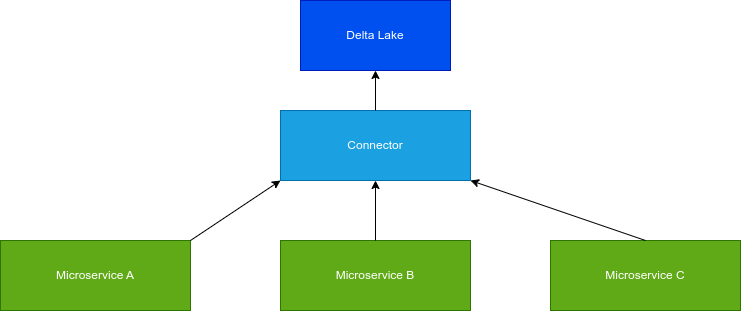
\includegraphics[width=\linewidth]{images/delta-lake-microservices.png}
\caption{Delta lake connectés à des microservices}\label{fig:schema-delta}
\end{figure}

\section{Côté Frontend}
Pour la mise en œuvre des microservices, nous avons décider d'utiliser Spring Boot, un framework Java populaire pour le développement d'applications. En utilisant Spring Boot, nous pouvons créer des microservices autonomes, indépendants les uns des autres, qui peuvent être développés, déployés et scalés individuellement. Spring Boot fournit également des fonctionnalités telles que la gestion de la persistance des données, la sécurité et la création d'API REST, ce qui facilite le développement des microservices.

\begin{figure}[H]
\centering
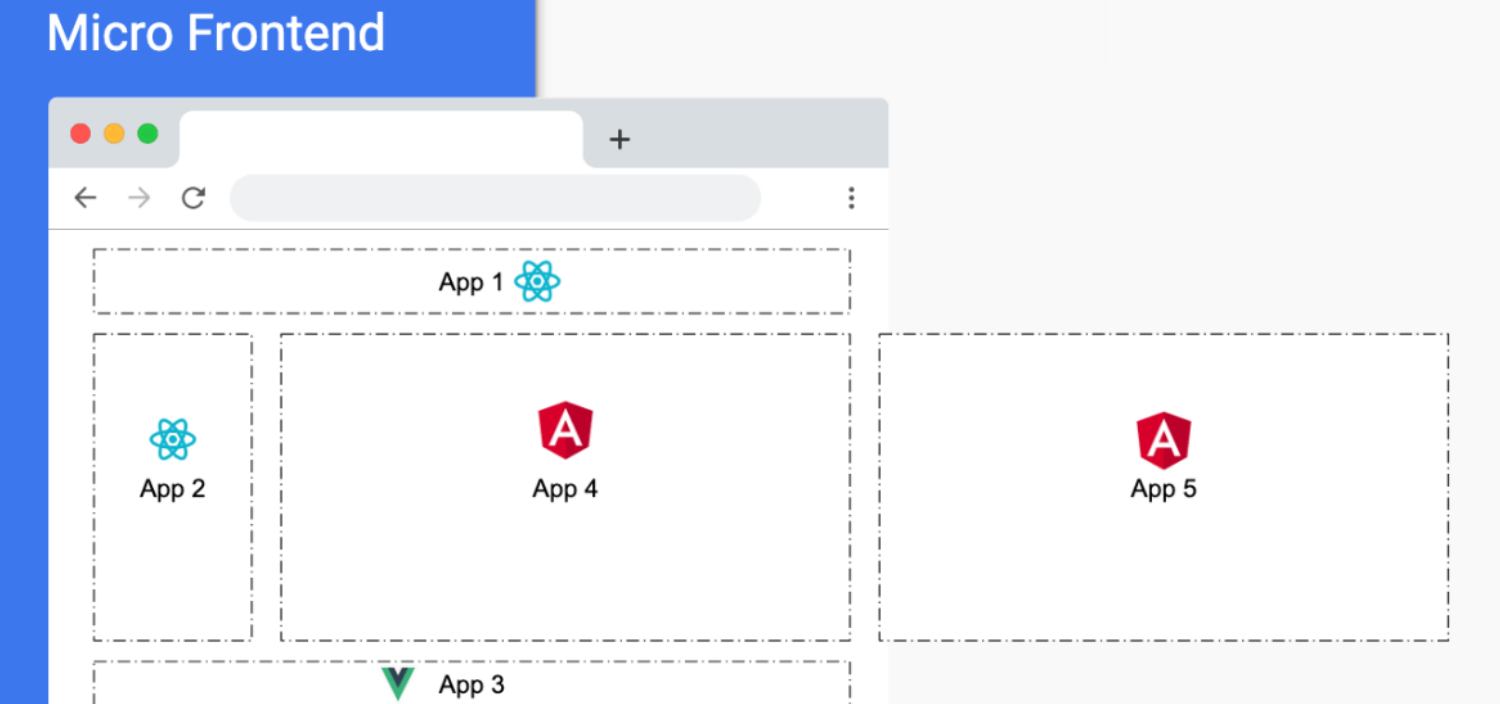
\includegraphics[width=\linewidth]{images/microfrontends.png}
\caption{Schéma des microfrontends}\label{fig:schema-microfrontends}
\end{figure}

\section*{Conclusion}
\addcontentsline{toc}{section}{Conclusion}

En adoptant ce cheminement de solution, nous visons à moderniser et à améliorer l'architecture de notre système. En remplaçant l'exporter worker et les bases de données MariaDB par Delta Lake sur le Cloud Object Store, nous assurons une meilleure gestion des données, scalable et moins chère. En utilisant des microservices avec Spring Boot, nous obtenons une architecture plus modulaire, évolutive et facile à maintenir du côté backend. Enfin, en utilisant des micro-frontends avec React, nous améliorons la flexibilité et la maintenabilité de l'interface utilisateur.